\documentclass[12pt,reqno]{amsart}
\usepackage{geometry} % see geometry.pdf on how to lay out the page. There's lots.
\geometry{a4paper} % or letter or a5paper or ... etc

\usepackage{graphicx}

\usepackage{nomencl}

\title{Inductive And Capacitive Coupling}
\author{Matthew Beck}
\date{\today}

%%% BEGIN DOCUMENT
\begin{document}
\maketitle
\makenomenclature
\setlength{\parindent}{0pt}

%$\omega$ $\text{P}_\text{App}$
\nomenclature{$\omega_r$}{Resonant cavity frequency}
\nomenclature{$M$}{Coupling Inductance}
\nomenclature{$C_c$}{Coupling Capacitance}
\nomenclature{$C_\text{Res}$}{Resonator Capacitance}
\nomenclature{$L_\text{Res}$}{Resonator Inductance}
\nomenclature{$Q_c^L$}{Inductive Coupling quality factor}
\nomenclature{$Q_c^C$}{Capacitive coupling quality factor}
\printnomenclature[6cm]

\section*{Inductive Coupling}

\begin{figure}[h!]
\begin{center}
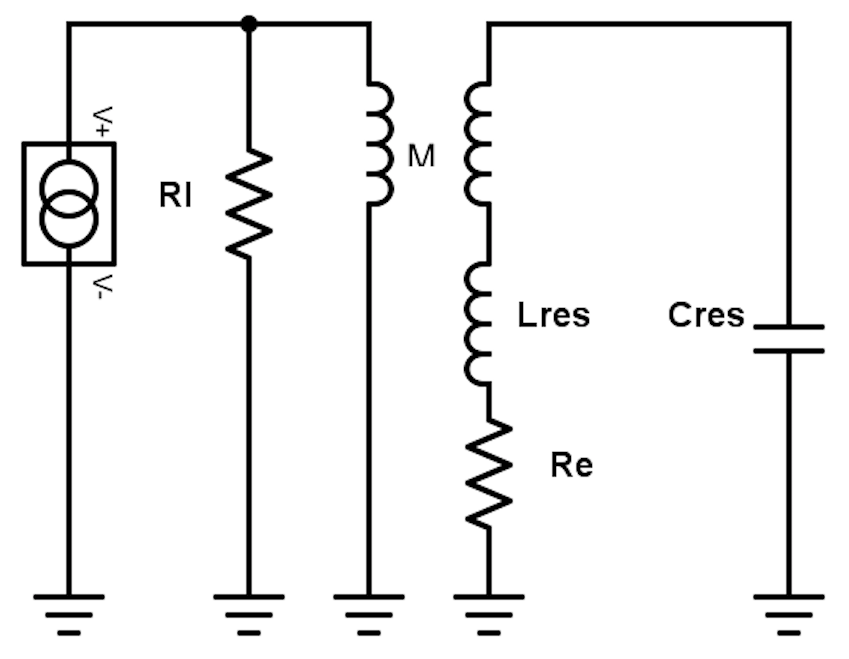
\includegraphics[scale = 0.25]{Lcoupling.png}
\end{center}
\end{figure}

We begin by defining the noise current power spectral density for the input side of the circuit.

\begin{equation}
S_I = \frac{4k_bT}{R_l}
\label{LcoupSI}
\end{equation}

The induced noise voltage on the resonator is then

\begin{equation}
S_V = 4k_bTR_e
\label{LcoupSv}
\end{equation}

We can relate \eqref{LcoupSI} and \eqref{LcoupSv} via the mutual inductance, M and the frequency.

\begin{equation}
\frac{4k_bT}{R_l}(\omega M)^2 = 4k_bTR_e
\end{equation}

Solving for $R_e$ yields

\begin{equation}
Re = \frac{(\omega M)^2}{R_l}
\end{equation}

The inductive coupling quality factor is then defined as

\begin{equation}
Q_c^L = \frac{\omega L_\text{res}}{R_e} = \frac{L_\text{res} R_l}{\omega M^2} = \frac{2 Z_0 L_\text{res}}{\omega M^2}
\end{equation}

Where the substitution $R_l = 2Z_0$ has been made.

\section*{Capacitive Coupling}

\begin{figure}[h!]
\begin{center}
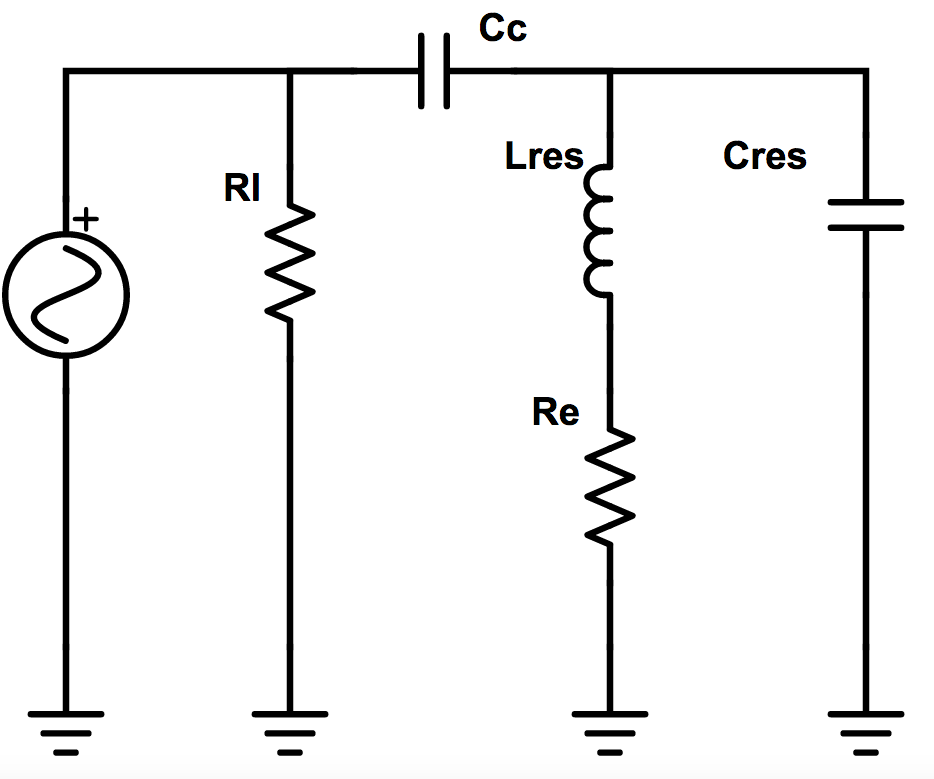
\includegraphics[scale = 0.25]{Ccoupling.png}
\end{center}
\end{figure}

We begin by defining the noise voltage power spectral density for the input side of the circuit

\begin{equation}
S_V = 4k_bT R_l
\label{CcoupSv}
\end{equation}

This induces a noise current in the resonator of the form

\begin{equation}
S_I = \frac{4k_bT}{R_e}
\label{CcoupSI}
\end{equation}

This can be equated via the coupling impedance

\begin{align}
\frac{S_I}{(\omega C_c)^2} &= S_V \\
\frac{4k_bT}{R_e(\omega C_c)^2} &= 4k_bTR_l \\
R_e &= \frac{1}{(\omega C_c)^2R_l}
\end{align}

We can then define the coupling quality factor as

\begin{align}
Q_c^C  &= \omega R_e C \\ 
&= \frac{\omega C}{(\omega C_c)^2 R_l} \\ 
&= \frac{C}{2Z_0 \omega C_c^2} \label{Qc}
\end{align}

Where we have again made the substitution $R_l = 2Z_0$. One can see that \eqref{Qc} matches with the result obtained in Goppl, et al. in the limit that $(\omega C_c R_l)^2 \ll 1$


\end{document}